\chapter{ModeloDinamico}	


	Este capítulo describe en modelo dinámico del sistema. en el se detallan todos los escenarios de ejecución del sistema. La figura~\ref{fig:casosDeUso} muestra el diagrama general del sistema y todos sus casos de uso.

%---------------------------------------------------------
\section{Descripción de actores}

%---------------------------------------------------------DUEÑO
\begin{Usuario}{\hypertarget{Dueño}{\subsection{Dueño}}}{
	Es el encargado de todas las operaciones de mayor importancia de las farmacias
	se encarga de contratar al personal, tanto empleados como supervisores y también controla las sucursales de la farmacia.
}
    \item[Responsabilidades:] \cdtEmpty
    \begin{itemize}
		\item Contratar Personal y asignarlo a una sucursal.
		\item Asignar  sucursales.
		\item Crear paquetes de descuento.
		\item Dar de baja Personal.
		\item Cerrar sucursales.
		\item Agregar nuevos tipos de medicamentos al sistema.
		\item Dar de baja paquetes de descuento.
		\item Modificar los medicamentos en los paquetes de descuento.
		\item Controlar los permisos en el sistema.
		\item Conocer al personal.	
    \end{itemize}
\end{Usuario}

%---------------------------------------------------------Supervisor
\begin{Usuario}{\hypertarget{Supervisor}{\subsection{Supervisor}}}{
	Es el encargado de llevar un control de la apertura y cierre de turno,
	así como hacer un reporte de ventas mensuales al dueño sobre las sucursales en las que esta asignado.
}
    \item[Responsabilidades:] \cdtEmpty
    \begin{itemize}
		\item Dar de baja medicamentos estropeados.
		\item Supervisar a los empleados.
		\item Abrir turno del cajero.
		\item Cerrar turno del cajero.
		\item Cambiar los datos de los medicamentos que estén registrados de forma incorrecta.
    \end{itemize}
    
	\item[Perfil:] \cdtEmpty
    \begin{itemize}
		\item Amplia experiencia en el rama de farmacias.
		\item Licenciatura como mínimo.
    \end{itemize}
\end{Usuario}

%---------------------------------------------------------Empleado
\begin{Usuario}{\hypertarget{Empleado}{\subsection{Cajero}}}{
	Es el encargado de realizar la ventas, atender proveedores y clientes
}
    \item[Responsabilidades:] \cdtEmpty
    \begin{itemize}
		\item Registra medicamentos del proveedor.
		\item Realiza ventas.
		\item Aplica descuentos de los paquetes hechos por el dueño.
		\item Registrar datos de clientes en el sistema.
		\item Hacer devoluciones.
		\item Dar créditos al cliente con los cuales se puede comprar medicina.
		\item Conocer los medicamentos que se tienen en su sucursal a si como la cantidad de cada medicamento.
    \end{itemize}

	\item[Perfil:] \cdtEmpty
    \begin{itemize}
		\item Bachillerato terminado.
		\item Responsable
		\item Honesto
    \end{itemize}
\end{Usuario}
A continuación se detallan los casos de uso.

%---------------------------------------------------------
\begin{figure}[htbp]
	\begin{center}
		\fbox{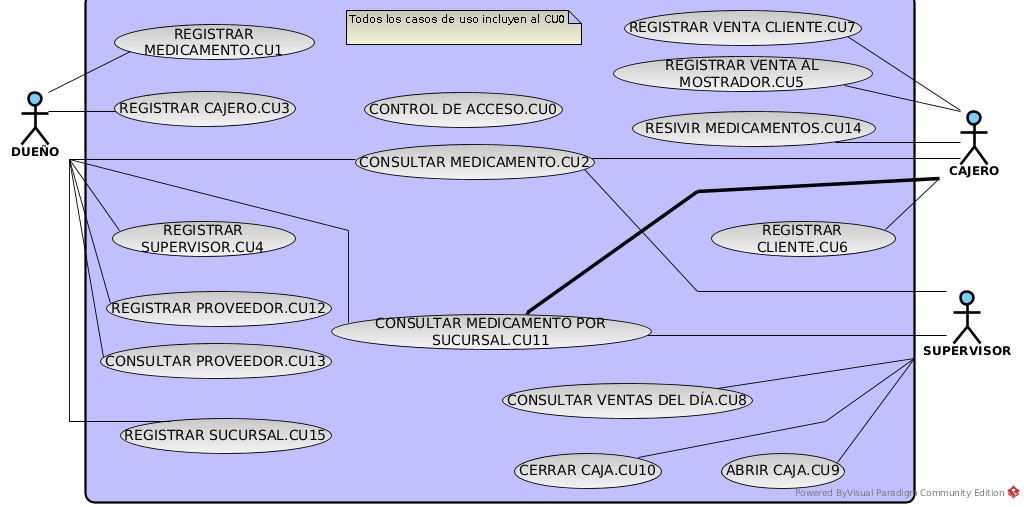
\includegraphics[width=18cm, height=20cm]{images/DiagramaCU}}
		\caption{Diagrama de casos de uso del sistema.}
		\label{fig:casosDeUso}
	\end{center}
\end{figure}
\begin{figure}[htbp]
	\begin{center}
		\fbox{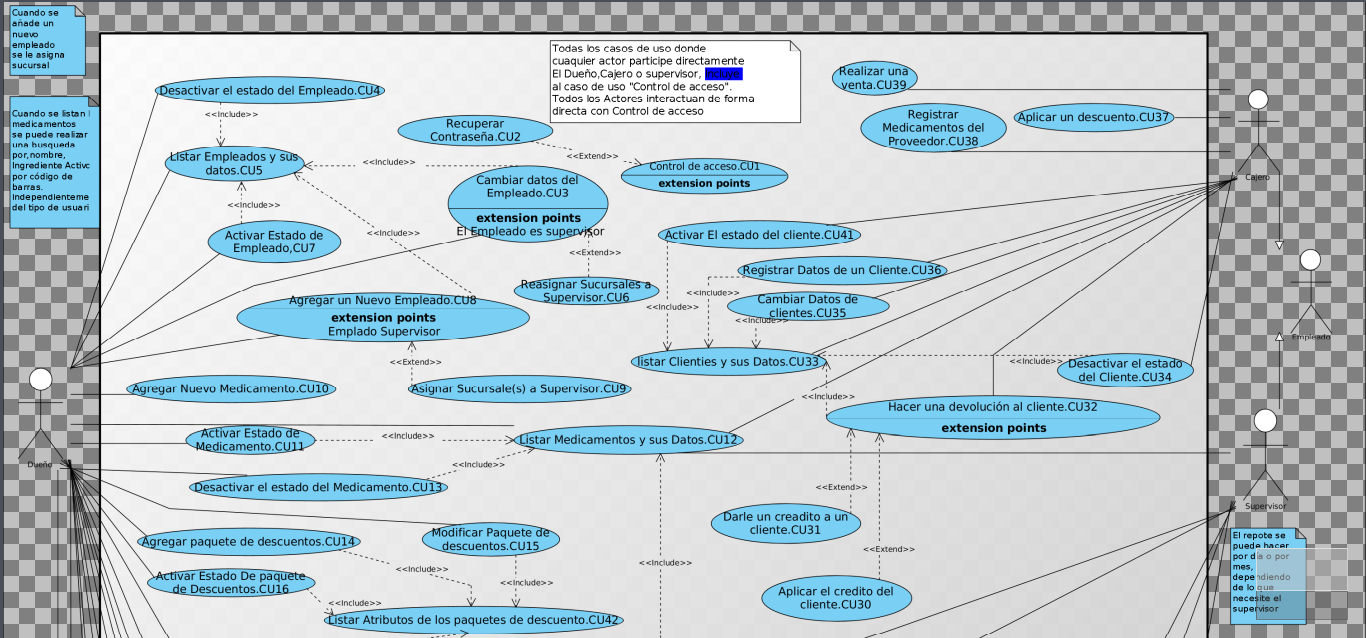
\includegraphics[width=18cm, height=20cm]{images/Diagrama1}}
		\caption{Diagrama de casos de uso del sistema parte de arriba.}
		\label{fig:casosDeUso}
	\end{center}
\end{figure}

\begin{figure}[htbp]
	\begin{center}
		\fbox{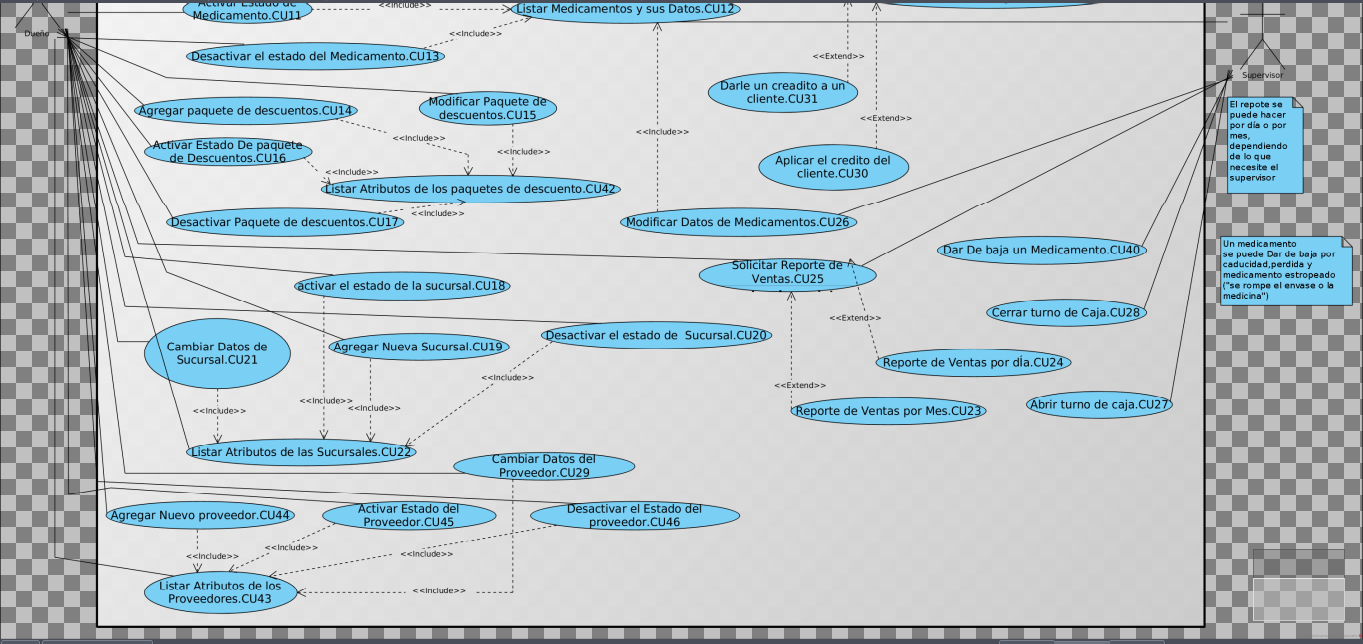
\includegraphics[width=18cm, height=20cm]{images/Diagrama2}}
		\caption{Diagrama de casos de uso del sistema parte de abajo.}
		\label{fig:casosDeUso}
	\end{center}
\end{figure}
%CASOS DE USO
Esencia de los Casos de Uso.
 \begin{UseCase}{CU1}{Registro de medicamento}{
		El Dueño es el unico actor que puede hacer un registro de un medicamento en el sistema.
	}
		\UCitem{Versión}{\color{Gray}0.1}
		\UCitem{Autor}{\color{Gray}Felipe Zamora Gachuz}
		\UCitem{Supervisa}{\color{Gray}.}
		\UCitem{Actor}{Dueño}
		\UCitem{Propósito}{El dueño registra un nuevo medicamento en el sistema para poeder hacer las ventas porteriores}
		\UCitem{Entradas}{Datos del medicamento, datos del proveedor del medicamento}
		\UCitem{Origen}{Teclado}
		\UCitem{Salidas}{Registro en la base de datos del nuevo medicamento}
		\UCitem{Destino}{BD}
		\UCitem{Precondiciones}{No tener ya registrado el medicamento,tener registro del proveedor, estar en las pantallas del dueño. }
		\UCitem{Postcondiciones}{Registro del medicamento en el sistema}
		\UCitem{Errores}{Medicamento parecido  ya registrado, proveedor no encontrado}
		\UCitem{Observaciones}{}
		\UCitem{Estado}{En revision}
	\end{UseCase}
%--------------------------------------
	\begin{UCtrayectoria}{Principal}
		\UCpaso[\UCactor] Tiene que estar en las pantallas de dueño.
		\UCpaso [\UCactor]El abre el formulario de registro de medicamentos. 
		\UCpaso El sistema despliega la pantalla \IUref{IU5}{FormularioMedicamento} \Trayref{D}.%CANCELAR OPERACION
		\UCpaso [\UCactor] Tiene que llenar los datos solicitados del medicamento y proveedor.%\Trayref{A}
		\UCpaso El sistema verifica el formulario este llenado(no este vacio) \Trayref{A},\Trayref{D}
		\UCpaso El sistema comprueba el proveedor este registrado \Trayref{B},\Trayref{D}
		\UCpaso El sistema registra el medicamento en el sistema con el proveedor indicado, mostrando la pantalla \IUref{MSG6}{ConfirmarOperación}.
		\UCpaso	[\UCactor]Preciona el boton aceptar.\Trayref{C},\Trayref{D}
		\UCpaso El sistema regresa a las pantallas del dueño.	
	\end{UCtrayectoria}

%--------------------------------------		
	\begin{UCtrayectoriaA}{A}{Hay datos en el formulario que estan vacios}
			\UCpaso El sistema muestra junto al campo vacio que el dato es necesario.
			\UCpaso Continúa en el paso 4 del \UCref{CU1}.
		\end{UCtrayectoriaA}
%----------------------------------------
		\begin{UCtrayectoriaA}{B}{No se encuentra el proveedor}
			\UCpaso El sistema muestra junto al campo del proveedor del medicamento que ese proveedor no se encuenta registrado.
			\UCpaso[] Continua en el paso 4 del \UCref{CU1}.
		\end{UCtrayectoriaA}		
%--------------------------------------
		\begin{UCtrayectoriaA}{C}{Preciona el boton cancelar}
			\UCpaso Continua en el paso 4 del \UCref{CU1}.
		\end{UCtrayectoriaA} % control de acceso
\begin{UseCase}{CU2}{Recuperar Contraseña}{
		El empleado puede cometer la equivocación de perder la contraseña asociada a la cuenta con la que ingresa al sistema, por lo cual se requiere de una forma para poder recuperar la contraseña. La recuperación de realizara mediante un correo electrónico el cual se le enviara al empleado con la posibilidad de reasignar una nueva contraseña
	}
		\UCitem{Versión}{\color{Gray}0.1}
		\UCitem{Autor}{\color{Gray}Enrique Aguilera Rosas Landa}
		\UCitem{Supervisa}{\color{Gray}Correa Medina Carlos Miguel}
		\UCitem{Actor}{\hyperlink{Empleado}{Supervisor, Cajero}}
		\UCitem{Propósito}{Conceder el acceso al sistema de nuevo mediante la recuperación de la contraseña.}
		\UCitem{Entradas}{Correo Electrónico.}
		\UCitem{Origen}{Teclado}
		\UCitem{Salidas}{Contraseña Asociada con la cuenta.}
		\UCitem{Destino}{Pantalla}
		\UCitem{Precondiciones}{El empleado debe estar registrado en el sistema y que no recuerde su contraseña asociada .}
		\UCitem{Postcondiciones}{El empleado recuperara su contraseña y su acceso al sistema.}
		\UCitem{Errores}{Que el acceso a la pagina sea incorrecto debido a razones de Errores De conexión o Mantenimiento de los Servidores, Que el usuario no este registrado en el sistema}

		\UCitem{Observaciones}{}
		\UCitem{Estado}{Corrección}
	\end{UseCase}
%--------------------------------------
	\begin{UCtrayectoria}{Principal}
		\UCpaso Incluye el caso de uso \UCref{CU1}.
		\UCpaso[\UCactor] Presiona el botón \IUbutton{¿Olvidaste tu Password?}.
		\UCpaso [\UCactor] Proporciona su Correo Electrónico asociado a la contraseña perdida y  Confirma la operación presionando el botón  \IUbutton{Aceptar}.		
		\UCpaso Verifica que el correo proporcionado cumpla con el formato ``Ejemplo@ejemplo.com'' \Trayref{A}
		\UCpaso Busca la cuenta asociada al correo ingresado. \Trayref{B}
		\UCpaso Verifica que dicha cuenta este activa. \Trayref{C}.
		\UCpaso Envía un correo electrónico al correo proporcionado; el cual contara con un link que lleva a la \IUref{12}{Recuperar Contraseña} para asignar una nueva contraseña. \Trayref{D}.
		\UCpaso Redirecciona al \UCactor a la  \IUref{IU1}{Pantalla Principal}.
	\end{UCtrayectoria}

%--------------------------------------		
	\begin{UCtrayectoriaA}{A}{El Correo no esta Correcto}
			\UCpaso Muestra el Mensaje {\bf MSG01-}``Error en la Operación [{\em correo con formato incorrecto}] Introduzca un correo con el formato xxx@xx.xx .''.
			\UCpaso Continúa en el paso 3 del \UCref{CU2}.
		\end{UCtrayectoriaA}
%----------------------------------------
		\begin{UCtrayectoriaA}{B}{El \UCactor no esta registrado}
			\UCpaso Muestra el Mensaje {\bf MSG01-}``Error en la operación [{\em Usuario no Encontrado}] El usuario y/o contraseña no existen .''.
			\UCpaso[\UCactor] Oprime el botón \IUbutton{Aceptar}.
			\UCpaso[] Continua en el paso 3 del \UCref{CU2}.
		\end{UCtrayectoriaA}		
%--------------------------------------
		\begin{UCtrayectoriaA}{C}{La cuenta a la que intenta acceder no esta activa}
			\UCpaso Muestra el Mensaje {\bf MSG01-}``Error en la operación [{\em Cuenta Desactivada}] Contacta con el Dueño para resolver el problema .''.
			\UCpaso[\UCactor] Oprime el botón \IUbutton{Aceptar}
			\UCpaso Continua en el paso 3 del \UCref{CU2}.
		\end{UCtrayectoriaA}
%--------------------------------------
	\begin{UCtrayectoriaA}{D}{Correo Electrónico de recuperación de contraseña no se envió}
			\UCpaso Muestra el Mensaje {\bf MSG01-}``Error en la operación [{\em Correo no enviado}] Revisa tu conexión y vuelve a enviar el mensaje .''.
			\UCpaso[\UCactor] Oprime el botón \IUbutton{Aceptar}
			\UCpaso Continua en el paso 7 del \UCref{CU2}.
		\end{UCtrayectoriaA}
%--------------------------------------


		
 % Recuperar Contaseña
\begin{UseCase}{CU3}{Registrar cajero}{
		El dueño es el unico que puede registrar un cajero en el sistema para las sucursales que lo requieran.
	}
		\UCitem{Versión}{\color{Gray}0.1.2}
		\UCitem{Autor}{\color{Gray}Felipe Zamora Gachuz}
		\UCitem{Supervisa}{\color{Gray} }
		\UCitem{Actor}{Dueño}
		\UCitem{Propósito}{Registrar cajeros en la sucursales donde faltan cajeros}
		\UCitem{Entradas}{Nombre, Apellidos del solicitante, telefono, salario, sucursal}
		\UCitem{Origen}{Teclado}
		\UCitem{Salidas}{Registro de un cajero en una unica sucursal}
		\UCitem{Destino}{BD}
		\UCitem{Precondiciones}{No tener dado de alta al cajero en el sistema en general}
		\UCitem{Postcondiciones}{Registro en el sistema de un cajero en una sucursal}
		\UCitem{Errores}{Exista algun duplicado en los datos del empleado, sus cambios no sean guardados}
		\UCitem{Observaciones}{El cajero siempre tiene asignado sucursal}
		\UCitem{Estado}{En revision}
	\end{UseCase}
%--------------------------------------
	\begin{UCtrayectoria}{Principal}
		\UCpaso [\UCactor] Tiene que estar en las pantallas de dueño.
		\UCpaso [\UCactor] El abre el formulario agregar cajero.
		\UCpaso El sistema despliega la pantalla \IUref{IU7}{FormulariCajero}.
		\UCpaso [\UCactor] Introduce los datos del formulario incluyendo la sucursal \Trayref{A},\Trayref{B},\Trayref{D}.%sucursal mal
		\UCpaso El sistema verifica los cajeros de la sucursal del paso anterior(verifica el numero de cajeros en la sucursal) \Trayref{C},\Trayref{D}.%muchos cajeros en sucursal
		\UCpaso [\UCactor]Preciona el boton aceptar \Trayref{D}.
		\UCpaso El sistema regresa a las pantallas del dueño.
	\end{UCtrayectoria}

\textbf{NOTA:El numero de cajeros y supervisores es de 3 por sucursal.}
%-------------------------------------------------------------------------


\begin{UCtrayectoriaA}{A}{Sucursal no encontrada}
			\UCpaso El sistema muestra junto al campo sucursal que no es valida.
			\UCpaso Continúa en el paso 4 del \UCref{CU3}.
		\end{UCtrayectoriaA}
%-------------------------------------------------------------------------


\begin{UCtrayectoriaA}{B}{Algun campo del Cajero tiene un error de formato.}
			\UCpaso El sistema muestra junto al campo del error, que es error de formato.
			\UCpaso Continúa en el paso 4 del \UCref{CU3}.
		\end{UCtrayectoriaA}
%-------------------------------------------------------------------------

\begin{UCtrayectoriaA}{C}{La sucursal valida seleccionada ya tiene los empleados necesarios para el horario de atención}
			\UCpaso El sistema muestra junto al campo sucursal que la sucursal ya tiene los empledos necesarios para el horario de atención.
			\UCpaso Continúa en el paso 4 del \UCref{CU3}.
		\end{UCtrayectoriaA}
%-------------------------------------------------------------------------


\begin{UCtrayectoriaA}{D}{Da en el boton cancelar}
		\UCpaso El sistema regresa a las pantallas del dueño.
\end{UCtrayectoriaA} % Cambiar datos de empleado
 \begin{UseCase}{CU4}{Registrar Supervisor}{
		Con el crecimiento de la Franquicia, es necesario contratar nuevo personal, personal encargado de administrar diferentes sucursales, este empleado es el supervisor,el mismo tiene responsabilidades en el sistema, por lo tanto el dueño  necesita de un método sencillo y rápido con el que le pueda incorporar al supervisor al trabajo una vez contratado.
	}
		\UCitem{Versión}{\color{Gray}0.1}
		\UCitem{Autor}{\color{Gray}Correa Medina Carlos Miguel}
		\UCitem{Supervisa}{\color{Gray}.Darwin}
		\UCitem{Actor}{Dueño}
		\UCitem{Propósito}{facilitar la incorporación de un nuevo supervisor, asignado áreas de trabajo de forma sencilla y eficaz.}
		\UCitem{Entradas}{Todos los datos proporcionados en el Formulario \IUref{IU2}{Formulario Supervisor}}
		\UCitem{Origen}{Teclado}
		\UCitem{Salidas}{nueva fila en  \IUref{IU13}{Tabla Supervisores}}
		\UCitem{Destino}{Pantalla}
		\UCitem{Precondiciones}{El Supervisor no debe estar registrado en el sistema,debe existir por lo menos una sucursal registrada en el sistema.}
		\UCitem{Postcondiciones}{la capacidad de supervisores por Sucursal disminuye en tres Sucursales máximo y solo una sucursal como mínimo.}
		\UCitem{Errores}{Que no se cuente con conexión a Internet,no haya energía eléctrica para utilizar un computador,Que no se realice una conexión a la base de datos,que el servidor se caiga,que los datos proporcionados estén erróneos, que no haya cupo en ninguna sucursal.}
		\UCitem{Viene de...}{\UCref{CU0}{Control de acceso}}
		\UCitem{Observaciones}{}
		\UCitem{Estado}{En revisión}
	\end{UseCase}
%--------------------------------------
	\begin{UCtrayectoria}{Principal}
		\UCpaso incluye al caso de uso \UCref{IU0}{Control de Acceso}.
		\UCpaso [\UCactor] presiona el botón \IUbutton{Empleados}
		\UCpaso verifica que los permisos de usuario sean permisos de Dueño. \Trayref{A}
		\UCpaso Despliega una lista con los botones \IUbutton{Supervisor} y 
		\IUbutton{Cajero}
		\UCpaso [\UCactor] presiona el botón \IUbutton{Supervisor}
		\UCpaso Muestra la pantalla \IUref{IU13}{Tabla supervisores}
		\UCpaso [\UCactor] Presiona el botón \IUbutton{+Nuevo}
		\UCpaso Genera una lista con los nombres de las Sucursales que hay están en el sistema y la muestra en \IUref{IU2}{Formulario Supervisor} como una ``checklist"
		\UCpaso Marca las ``checklist" ,generadas en el paso anterior, de las sucursales que ya no tienen cupo para más Supervisores y las des-habilita para no reasignar Sucursales.\Trayref{B} 	 	 
		\UCpaso Muestra la pantalla \IUref{IU2}{Formulario Supervisor}
		\UCpaso [\UCactor] llena los campos: nombre,Apellido Paterno,Apellido Materno, Email, Teléfono y Salario.
		\UCpaso [\UCactor] De las Sucursales desmarcadas selecciona las sucursales de las que se hará cargo el supervisor (máximo 3 mínimo 1)
		\UCpaso [\UCactor] Presiona el botón \IUbutton{Guardar}.
		\UCpaso Verifica que ningún campo del formulario este vació \Trayref{C}
		\UCpaso Verifica que el salario sea un dígito.\Trayref{D}
		\UCpaso Verifica que por lo menos este marcada una Sucursal más de las Sucursales marcadas generadas en el paso 9 de este caso de uso.\Trayref{F}
		\UCpaso Muestra la pantalla \IUref{IU13}{Tabla Supervisores}
	\end{UCtrayectoria}

%--------------------------------------		
	\begin{UCtrayectoriaA}{A}{Permiso Denegado}
			\UCpaso Muestra el Mensaje {\bf MSG4-}``Cancelado[{\em Permiso Denegado }].''.
			\UCpaso Muestra la pantalla \IUref{IU13}{Tabla Supervisores}.
		\end{UCtrayectoriaA}
%----------------------------------------
		\begin{UCtrayectoriaA}{B}{No hay ninguna Sucursal Registrada en el sistema }
			\UCpaso Muestra el Mensaje {\bf MSG1-}``Error en la operación [{\em No hay sucursales Registradas aun.}] antes de registrar a algún empleado es necesario que se registre por lo menos una Sucursal, o que exista una Sucursal con puestos vacantes.''.
			\UCpaso[\UCactor] Oprime el botón \IUbutton{ok}.
			\UCpaso Muestra la pantalla \IUref{IU13}{Tabla Supervisores}.
		\end{UCtrayectoriaA}		
%--------------------------------------
		\begin{UCtrayectoriaA}{C}{Existe por lo menos un campo obligatoria que esta vació}
			\UCpaso remarca con Rojo los campos obligatorios que están vacíos 
			y pone la leyenda ``Campo Obligatorio".
			\UCpaso Muestra el Mensaje {\bf MSG1-}``Error en la operación [{\em Campos obligatorios vacíos}] Los campos llenados con Rojo no pueden estar vacíos.''.
			\UCpaso[\UCactor] Oprime el botón \IUbutton{Aceptar}
			\UCpaso Regresa a la pantalla \IUref{IU2}{Formulario Supervisor} Mostrando los campos en rojo y dejando la información introducida en el paso 11 de este caso de uso, como se quedo.
		\end{UCtrayectoriaA}
%--------------------------------------
		\begin{UCtrayectoriaA}{D}{Tipo de Dato Incorrecto}
			\UCpaso remarca con rojo el campo que debe ser dígito, y muestra la leyenda ``Este campo debe ser un dígito" debajo del campo ``salario" en la  pantalla \IUref{IU2}{Formulario Supervisor}.
			\UCpaso Muestra el Mensaje {\bf MSG01-}``Error en la Operación [{\em Tipo de Dato Invalido}]En el campo salario solo se debe introducir números.''.
			\UCpaso Regresa a la pantalla \IUref{IU2}{Formulario Supervisor} Mostrando los campos en rojo y dejando la información introducida en el paso 11 de este caso de uso, como se quedo.
			\UCpaso Continua en el paso 11 de este caso de uso.
		\end{UCtrayectoriaA}
%--------------------------------------
		\begin{UCtrayectoriaA}{F}{Sucursales mal asignadas}
			\UCpaso Crea la leyenda ``Asigna por lo menos una Sucursal" en rojo y la coloca hasta abajo de la pantalla \IUref{IU2}{Formulario Supervisor}
			\UCpaso Muestra el Mensaje {\bf MSG1-}``Error en la Operación [{\em Asignación incorrecta de sucursal}]Verifica que por lo menos se le haya asignado una sucursal al supervisor que se esta registrando.''.
			\UCpaso Regresa a la pantalla \IUref{IU2}{Formulario Supervisor} Mostrando los campos en rojo y, dejando la información introducida en el paso 11 de este caso de uso, como la dejo el [\UCactor].
			\UCpaso Continua en el paso 11 de este caso de uso.
		\end{UCtrayectoriaA} % Desactivar el estado del empleado
\begin{UseCase}{CU5}{Listar Empleados y sus Datos}{
		La farmacia consta con múltiples empleados y para poder checar los datos de todos los empleados, la opción mas eficaz es hacer un listado con los empleados y sus datos correspondientes
	}
		\UCitem{Versión}{\color{Gray}0.1.3}
		\UCitem{Autor}{\color{Gray}Aguilera Rosas Landa Enrique}
		\UCitem{Supervisa}{\color{Gray}Correa Medina Carlos Miguel}
		\UCitem{Actor}{Dueño}
		\UCitem{Propósito}{Control rápido sobre el manejo de los datos de los empleados.}
		\UCitem{Entradas}{Nombre del Empleado, Id de Empleado}
		\UCitem{Origen}{Teclado}
		\UCitem{Salidas}{No Aplica.}
		\UCitem{Destino}{Pantalla}
		\UCitem{Precondiciones}{El empleado debe de estar registrado en el sistema.}
		\UCitem{Postcondiciones}{El dueño checara la lista de los empleados y sus respectivos datos .}
		\UCitem{Errores}{La pagina sea inaccesible por el momento debido a fallas con los servidores, Que el empleado tenga su cuenta no este registrado}
		\UCitem{Observaciones}{}
		\UCitem{Estado}{Revision}
	\end{UseCase}
%--------------------------------------
	\begin{UCtrayectoria}{Principal}
		\UCpaso Incluye el caso de uso \UCref{CU1} paso 11
		\UCpaso[\UCactor] Selecciona La opción de ver Lista de  Empleados presionando el botón \IUbutton{Empleados}.
		\UCpaso[\UCactor] Introduce el Nombre del empleado a buscar en el campo de Búsqueda y Presiona el \IUbutton{Buscar}.
		\UCpaso Genera y Despliega una lista que coincida con la búsqueda realizada. \Trayref{A} 
		\UCpaso [\UCactor] Presiona el \IUbutton{Regresar}.
		\UCpaso Redirige al [\UCactor] a la  \IUref{01}{Pantalla Principal}.
	\end{UCtrayectoria}


%-------------------------------------------------------------------------
\begin{UCtrayectoriaA}{A}{Empleado no encontrado.}
			\UCpaso Muestra el Mensaje {\bf MSG01-}``Error en la Operación [{\em Empleado no encontrado}] revisa que los campos sean llenados correctamente.''.
			\UCpaso Continúa en el paso 4 del \UCref{CU5}.
		\end{UCtrayectoriaA}
%-------------------------------------------------------------------------
 % Listar Empleados y sus datos 
\begin{UseCase}{CU6}{Reasignar Sucursales a Supervisor}{
		Un supervisor tiene la responsabilidad de checar el funcionamiento adecuado de las sucursales que le son asignadas y por lo tanto se le asignaran nuevas sucursales o se le modificaran dependiendo de los movimientos operacionales de cada una
	}
		\UCitem{Versión}{\color{Gray}0.1}
		\UCitem{Autor}{\color{Gray}Aguilera Rosas Landa Enrique}
		\UCitem{Supervisa}{\color{Gray}Correa Medican Carlos Miguel}
		\UCitem{Actor}{\hyperlink{Alumno}{Dueño}}
		\UCitem{Propósito}{Mejorar las operaciones diarias de la farmacia mediante resignaciones de supervisores adecuados.}
		\UCitem{Entradas}{Nombre del Empleado, Id de Empleado}
		\UCitem{Origen}{Teclado}
		\UCitem{Salidas}{No Aplica.}
		\UCitem{Destino}{Pantalla}
		\UCitem{Precondiciones}{El supervisor debe de estar registrado en el sistema y con un estado activado.}
		\UCitem{Postcondiciones}{ El supervisor por lo menos tendrá una sucursal diferente a la original .}
		\UCitem{Errores}{La pagina sea inaccesible por el momento debido a fallas con los servidores, Que el empleado tenga su cuenta desactivada}
		\UCitem{Observaciones}{ referencia a las IUX}
		\UCitem{Estado}{En Corrección}
	\end{UseCase}
%--------------------------------------
	\begin{UCtrayectoria}{Principal}
		\UCpaso Se extiende del caso de uso \UCref{CU3} paso 8
		\UCpaso [\UCactor] Modifica la sucursal del empleado y guarda los cambios presionando el botón\IUbutton{Aceptar y Guardar}
		\UCpaso Redirige al [\UCactor] a la  \IUref{01}{Pantalla Principal}.
	\end{UCtrayectoria}


%-------------------------------------------------------------------------
\begin{UCtrayectoriaA}{A}{Empleado no encontrado.}
			\UCpaso Muestra el Mensaje {\bf MSG01-}``Error en la Operación [{\em Empleado no encontrado}] revisa que los campos sean llenados correctamente.''.
			\UCpaso Continúa en el paso 4 del \UCref{CU4}.
		\end{UCtrayectoriaA}
%-------------------------------------------------------------------------
 % Reasignar Sucursales a supervisor
 \begin{UseCase}{CU5}{Registrar Venta Cliente}{
	Se necesita una manera fácil para poder registrar ventas a los clientes de cada sucursal, con fines de posibles aclaraciones o dudas que puedan surgir debio a los productos que ofrecemos.
	}
		\UCitem{Versión}{\color{Gray}0.1}
		\UCitem{Autor}{\color{Gray}Vázquez Cruz Fernando Darwin }
		\UCitem{Supervisa}{\color{Gray} Enrique Aguilera}
		\UCitem{Actor}{Cajero}
		\UCitem{Propósito}{Tener un control de las salidas de medicamento por ventas a clientes, para fines de cualquier aclaración o duda por parte del cliente.}
		\UCitem{Entradas}{Todos los datos requeridos en el formulario \IUref{IU19}{Formulario Venta}}
		\UCitem{Origen}{Teclado, mouse, lector de código de barras}
		\UCitem{Salidas}{comprobante de venta, salidas de medicamento(s)}
		\UCitem{Destino}{Pantalla,impresora}
		\UCitem{Precondiciones}{Los medicamentos a vender deben estar registrados en el sistema, el supervisor debió abrir la caja con anterioridad \UCref{CU9}{Abrir Caja}.}
		\UCitem{Postcondiciones}{Disminuye la cantidad de los medicamentos que se vendieron, se tiene una venta más registrada en el sistema a nombre de un cliente.}
		\UCitem{Errores}{Que no se realice una conexión a la base de datos,que el servidor se caiga,que los datos proporcionados estén erróneos, que el o los medicamentos estén registrados en el sistema pero no estén disponibles en la sucursal.}
		\UCitem{viene de...}{\UCref{CU0}{Control de acceso}}
		\UCitem{Observaciones}{}
		\UCitem{Estado}{En revisión}
	\end{UseCase}
%--------------------------------------
	\begin{UCtrayectoria}{Principal}
		\UCpaso [\UCactor] Presiona el botón \IUbutton{Ventas} que esta en la pantalla principal \IUref{IU1}{Pantalla principal}
		\UCpaso Verifica que los permisos de usuario sean permisos de cajero. \Trayref{A}
		\UCpaso Despliega el Formulario \IUref{IU19}{Formulario Ventas}.
		\UCpaso Busca el id del cajero que esta actualmente con la sesión activa y llena el campo "Empleado" con esa id.
		\UCpaso [\UCactor] En el primer campo de formulario "Cliente" Selecciona la opción "Cliente Preferente".
		\UCpaso Identifica la opción seleccionada por el [\UCactor] y despliega una checklist con los nombres de los clientes registrados en el sistema.
		\UCpaso [\UCactor] Da clic en donde esta el nombre del cliente al que se le registrará la venta.\Trayref{B}
		\UCpaso Llena el campo Cliente con el nombre seleccionado en el paso anterior. 
		\UCpaso [\UCactor] Escanea el código de barras del medicamento con el lector de código de barras.
		\UCpaso Llena el campo de `"Medicamentos" con el código de barras que se introdujo del lector.\Trayref{C}.
		\UCpaso Recibe un "Enter" del lector de código de barras y añade otra fila para agregar un nuevo medicamento en el campo "Medicamentos".
		\UCpaso Agrega en una lista que crea temporalmente, el nombre del  medicamento y el precio de venta del medicamento que fue leído por el lector de código de barras.
		\UCpaso Muestra la lista temporal de los medicamentos en el campo "Desglose de medicamentos y precios".\Trayref{D}
		\UCpaso Calcula el Total de los precios de venta de los medicamentos en la lista temporal y muestra la cantidad en el campo "Valor Total".
		\UCpaso [\UCactor] Presiona el botón \IUbutton{Guardar}.
		\UCpaso Muestra el Mensaje {\bf MSG6-}"Confirmar[{\em Confirmar Operación }]¿Los datos del formulario son correctos?.".
		\UCpaso [\UCactor] Presiona el botón \IUbutton{Aceptar}
		\UCpaso Verifica que ningún campo del formulario esté vació. \Trayref{E}
		\UCpaso Guarda los datos de la venta y actualiza la base de datos.
		\UCpaso Muestra el Mensaje {\bf MSG0-}"Exito[{\em Operación Realizada con exito }].".
		\UCpaso Muestra la pantalla \IUref{IU1}{Pantalla Principal}.
	\end{UCtrayectoria}

%--------------------------------------		
	\begin{UCtrayectoriaA}{A}{Permiso Denegado}
			\UCpaso Muestra el Mensaje {\bf MSG4-}`"Cancelado[{\em Permiso Denegado }].".
			\UCpaso Muestra la pantalla \IUref{IU1}{Pantalla Principal}.
		\end{UCtrayectoriaA}

%--------------------------------------
		\begin{UCtrayectoriaA}{B}{El cajero no encuetra el nombre del cliente}
			\UCpaso [\UCactor] Busca el nombre del cliente en el checklist pero no lo encuentra. 
			\UCpaso [\UCactor] Verifica la información proporcionada por le cliente.
			\UCpaso [\UCactor] Continua en el paso 5 de este caso de uso.			
		\end{UCtrayectoriaA}
		%--------------------------------------
		\begin{UCtrayectoriaA}{C}{El lector de barras no pudo leer bien el código}
			\UCpaso sigue su ejecución sin llenar el campo "Medicamentos""
			\UCpaso Continua en el paso 9 de este caso de uso.	
		\end{UCtrayectoriaA}
%----------------------------------------
		\begin{UCtrayectoriaA}{D}{Lista de medicamentos muy larga }
			\UCpaso Muestra en el formulario \IUref{IU19}{Formulario Ventas} un "scroll" en el campo de `"Desglose de medicamentos y precios"
			\UCpaso Regresa al paso 13 de este caso de uso.
		\end{UCtrayectoriaA}		
%--------------------------------------
			\begin{UCtrayectoriaA}{E}{Existe por lo menos un campo obligatorio que esta vacío}
			\UCpaso Remarca con Rojo los campos obligatorios que están vacíos y pone la leyenda "Campo Obligatorio".
			\UCpaso Muestra el Mensaje {\bf MSG1-}"Error en la operación [{\em Campos obligatorios vacíos}] Los campos llenados con Rojo no pueden estar vacíos.".
			\UCpaso[\UCactor] Oprime el botón \IUbutton{Aceptar}
			\UCpaso Regresa a la pantalla \IUref{IU19}{Formulario Ventas} Mostrando los campos en rojo y dejando la información introducida por el [\UCactor] en los pasos anteriores de este casos de uso
		\end{UCtrayectoriaA}
 % Activar estado de empleado
\begin{UseCase}{CU15}{Modificar paquete de descuento}{
		Realizar cambios en los paquetes de descuento.
	}
		\UCitem{Versión}{\color{Gray}0.1.2}
		\UCitem{Autor}{\color{Gray}Zapata Jasso José Rodolfo}
		\UCitem{Supervisa}{\color{Gray}Correa Medina Carlos Miguel}
		\UCitem{Actor}{\hyperlink{Alumno}{Dueño}}
		\UCitem{Propósito}{Realizar cambios en los paquetes de descuentos ya publicados.}
		\UCitem{Entradas}{Nombre del Empleado, Id de Empleado}
		\UCitem{Origen}{Teclado}
		\UCitem{Salidas}{No Aplica.}
		\UCitem{Destino}{Pantalla}
		\UCitem{Precondiciones}{Debe existir un paquete de descuento registrado previamente.}
		\UCitem{Postcondiciones}{El paquete de descuento deberá cambiar a como estaba previamente.}
		\UCitem{Errores}{La pagina sera inaccesible por el momento debido a fallas con los servidores, problemas al registrar cambios ne los paquetes.}
		\UCitem{Tipo}{Caso de uso primario}
		\UCitem{Observaciones}{}
		\UCitem{Estado}{Aprobado}
	\end{UseCase}


%--------------------------------------


	\begin{UCtrayectoria}{Principal}
		\UCpaso Se incluye el caso de uso \UCref{CU1}.
		\UCpaso Se incluye el caso de uso \UCref{Cu42} 
		\UCpaso[\UCactor] Selecciona la opción editar paquetes de descuento presionando el botón \IUref{IU11}{boton editar} que esta representado con un lapiz amarillo.
		\UCpaso Genera y Despliega el paquete de descuentos para su edición. 
		\UCpaso[\UCactor] Realiza los cambios que desea modificar en el paquete de descuentos y confirma al presiona el botón \IUbutton{Actualizar} . \Trayref{A}
		\UCpaso Redirige al [\UCactor] a la  \IUref{01}{Pantalla Principal de Dueno}.
	\end{UCtrayectoria}


%-------------------------------------------------------------------------


\begin{UCtrayectoriaA}{C}{Algun campo tiene un error.}
			\UCpaso Muestra el Mensaje {\bf MSG1-}`` [{\em Hubo un error en la operación }] revisa que los campos sean llenados correctamente.''.
			
		\end{UCtrayectoriaA}
 % Modificar paquete de descuento
\begin{UseCase}{CU16}{Activar estado de paquete de descuento}{
		Por razones laborales, es mejor activar el estado de un paquete de descuentos cuando sea necesario.
	}
		\UCitem{Versión}{\color{Gray}0.1.2}
		\UCitem{Autor}{\color{Gray}Zapata Jasso José Rodolfo}
		\UCitem{Supervisa}{\color{Gray}}
		\UCitem{Actor}{\hyperlink{Alumno}{Dueño}}
		\UCitem{Propósito}{Permitir realizar cambios en los paquetes de descuentos.}
		\UCitem{Entradas}{Nombre del Empleado, Id de Empleado}
		\UCitem{Origen}{Teclado}
		\UCitem{Salidas}{No Aplica.}
		\UCitem{Destino}{Pantalla}
		\UCitem{Precondiciones}{Debe existir un paquete de descuento registrado previamente y deberá estar desactivado.}
		\UCitem{Postcondiciones}{El paquete de descuento debera cambiar de desactivado a activado.}
		\UCitem{Errores}{La pagina sera inaccedible por el momento debido a fallas con los servidores.}
		\UCitem{Tipo}{Caso de uso secundario}
		\UCitem{Observaciones}{}
		\UCitem{Estado}{En revision}
	\end{UseCase}


%--------------------------------------


	\begin{UCtrayectoria}{Principal}
		\UCpaso Se extiende del caso de uso \UCref{CU0} paso 11
		\UCpaso[\UCactor] Selecciona la opción paquetes de descuento presionando el boton \IUbutton{Paquetes de descuento}.
		\UCpaso Lista los paquetes de descuento que estan registrados. 
		\UCpaso[\UCactor] Selecciona la opcion Activar estado, del paquete de descuentos que desea activar presionando el boton \IUbutton{Activar} que esta representado con una palomita azul.		
		\UCpaso Genera y despliega una pantalla de confirmación.  {\bf MSG3-}.
		\UCpaso[\UCactor] Confirma la acción seleccionando el boton\IUbutton{Si, Activar} . \Trayref{A}
		\UCpaso Guarda los cambios y redirige al [\UCactor] a la  \IUref{01}{Pantalla Principal de Dueno}.
	\end{UCtrayectoria}


%-------------------------------------------------------------------------


\begin{UCtrayectoriaA}{A}{Error al cambiar el estado.}
			\UCpaso Muestra el Mensaje {\bf MSG1-}`` [{\em Hubo un error en la operación}] ''.
			
		\end{UCtrayectoriaA}
%-------------------------------------------------------------------------

 % Activar estado de paquete de descuento
\begin{UseCase}{CU17}{Desactivar estado de paquete de descuento}{
		Por razones laborales, es mejor desactivar el estado de un paquete de descuentos en ves de eliminarlo.
	}
		\UCitem{Versión}{\color{Gray}0.1.2}
		\UCitem{Autor}{\color{Gray}Zapata Jasso José Rodolfo}
		\UCitem{Supervisa}{\color{Gray}Correa Medina Carlos Miguel}
		\UCitem{Actor}{\hyperlink{Alumno}{Dueño}}
		\UCitem{Propósito}{Evitar realizar cambios en los paquetes de descuentos cuando no sea necesario.}
		\UCitem{Entradas}{Nombre del Empleado, Id de Empleado}
		\UCitem{Origen}{Teclado}
		\UCitem{Salidas}{No Aplica.}
		\UCitem{Destino}{Pantalla}
		\UCitem{Precondiciones}{Debe existir un paquete de descuento registrado previamente y deberá estar activado.}
		\UCitem{Postcondiciones}{El paquete de descuento deberá cambiar de activado a desactivado.}
		\UCitem{Errores}{La pagina sera inaccesible por el momento debido a fallas con los servidores.}
		\UCitem{Tipo}{Caso de uso secundario}
		\UCitem{Observaciones}{}
		\UCitem{Estado}{Aprobado}
	\end{UseCase}


%--------------------------------------


	\begin{UCtrayectoria}{Principal}
		\UCpaso Se incluye el caso de uso \UCref{CU1}.
		\UCpaso Se incluye el caso de uso \UCref{CU42}.
		\UCpaso[\UCactor] Selecciona la opción Desactivar estado, del paquete de descuentos que desea desactivar presionando el botón \IUref{IU9}{boton desactivar} que esta representado con un bote de basura rojo.		
		\UCpaso Genera y despliega una pantalla de confirmación.  {\bf MSG3-} .
		\UCpaso[\UCactor] Confirma la acción seleccionando el botón\IUbutton{Si, Desactivar} . \Trayref{A}
		\UCpaso Guarda los cambios y redirige al [\UCactor] a la  \IUref{01}{Pantalla Principal de Dueño}.
	\end{UCtrayectoria}


%-------------------------------------------------------------------------


\begin{UCtrayectoriaA}{A}{Error al cambiar el estado.}
			\UCpaso Muestra el Mensaje {\bf MSG1-}`` [{\em Hubo un error en la operación}] ''.
			
		\end{UCtrayectoriaA}
%-------------------------------------------------------------------------
		 % Desactivar estado de paquete de descuento
\begin{UseCase}{CU18}{Activar estado de sucursal}{
		Se activa cuando la sucursal esta en operación.
	}
		\UCitem{Versión}{\color{Gray}0.1.2}
		\UCitem{Autor}{\color{Gray}Zapata Jasso José Rodolfo}
		\UCitem{Supervisa}{\color{Gray}Correa Medina Carlos Miguel}
		\UCitem{Actor}{\hyperlink{Alumno}{Dueño}}
		\UCitem{Propósito}{Disponibilidad de administrar la sucursal cuando esta en operación.}
		\UCitem{Entradas}{Nombre del Empleado, Id de Empleado}
		\UCitem{Origen}{Teclado}
		\UCitem{Salidas}{No Aplica.}
		\UCitem{Destino}{Pantalla}
		\UCitem{Precondiciones}{Debe existir dicha sucursal y debe estar desactivada.}
		\UCitem{Postcondiciones}{El estado de la sucursal deberá cambiar de desactivada a activada.}
		\UCitem{Errores}{La pagina sera inaccesible por el momento debido a fallas con los servidores.}
		\UCitem{Tipo}{Caso de uso primario}
		\UCitem{Observaciones}{}
		\UCitem{Estado}{Aprobado}
	\end{UseCase}


%--------------------------------------


	\begin{UCtrayectoria}{Principal}
		\UCpaso Se incluye el caso de uso \UCref{CU1}.
		\UCpaso Se incluye el caso de uso \UCref{CU22}
		\UCpaso[\UCactor] Selecciona la  Activar sucursal, de la sucursal que desea activar presionando el \IUref{IU10}{boton activar} que esta representado con una palomita azul.		
		\UCpaso Genera y despliega una pantalla de confirmación.  {\bf MSG3-}.
		\UCpaso[\UCactor] Confirma la acción seleccionando el botón\IUbutton{Si, Activar} . \Trayref{A}
		\UCpaso Guarda los cambios y redirige al [\UCactor] a la  \IUref{01}{Pantalla Principal de Dueño}.
	\end{UCtrayectoria}


%-------------------------------------------------------------------------


\begin{UCtrayectoriaA}{A}{Error al cambiar el estado.}
			\UCpaso Muestra el Mensaje {\bf MSG1-}`` [{\em error en la operación}] ''.
			
		\end{UCtrayectoriaA}
%-------------------------------------------------------------------------

 % Activar el estado de la sucursal
\begin{UseCase}{CU19}{Agregar nueva sucursal}{
		Registra una nueva sucursal para tener el control de está.
	}
		\UCitem{Versión}{\color{Gray}0.1.2}
		\UCitem{Autor}{\color{Gray}Zapata Jasso José Rodolfo}
		\UCitem{Supervisa}{\color{Gray}}
		\UCitem{Actor}{\hyperlink{Alumno}{Dueño}}
		\UCitem{Propósito}{Tener el control de una nueva sucursal cuando está este disponible para operar.}
		\UCitem{Entradas}{Nombre del Empleado, Id de Empleado}
		\UCitem{Origen}{Teclado}
		\UCitem{Salidas}{No Aplica.}
		\UCitem{Destino}{Pantalla}
		\UCitem{Precondiciones}{Debe haber una sucursal nueva fisica, que aun no este registrada en el sistema.}
		\UCitem{Postcondiciones}{Aparecera una nueva sucursal en el sistema.}
		\UCitem{Errores}{La pagina sera inaccedible por el momento debido a fallas con los servidores.}
		\UCitem{Tipo}{Caso de uso primario}
		\UCitem{Observaciones}{}
		\UCitem{Estado}{En revision}
	\end{UseCase}


%--------------------------------------


	\begin{UCtrayectoria}{Principal}
		\UCpaso Se extiende del caso de uso \UCref{CU0} paso 11

		\UCpaso[\UCactor] Selecciona la opcion Sucursales presionando el boton \IUbutton{Sucursales}.
		\UCpaso Dspliega la pantalla de Sucursales.
		\UCpaso[\UCactor] Selecciona la opcion Registar sucursal presionando el boton \IUbutton{Registar sucursal}.
		\UCpaso Genera un formulario para registrar una nueva sucursal. 
		\UCpaso[\UCactor] Llena los datos de formulario de manera que cada dato corresponda con la información que se pide y selecciona el boton \IUbutton{Guardar} .
		\UCpaso Genera y despliega una ventana emergente para confirmar. \Trayref{A}
		\UCpaso [\UCactor] Confirma la operación presionando el \IUbutton{Aceptar}
		\UCpaso Redirige al [\UCactor] a la  \IUref{01}{Pantalla Principal de Dueno}.
	\end{UCtrayectoria}


%-------------------------------------------------------------------------


\begin{UCtrayectoriaA}{A}{Problemas al guardar la sucursal.}
			\UCpaso Muestra el Mensaje {\bf MSG8-}`` [{\em Problemas al registar la sucursal}]Verifique los datos ''.
			
		\end{UCtrayectoriaA}
%-------------------------------------------------------------------------

 % Agregar nueva sucursal
\begin{UseCase}{CU20}{Desactivar estado de sucursal}{
		Se desactiva cuando la sucursal no estara en operación.
	}
		\UCitem{Versión}{\color{Gray}0.1.2}
		\UCitem{Autor}{\color{Gray}Zapata Jasso José Rodolfo}
		\UCitem{Supervisa}{\color{Gray}}
		\UCitem{Actor}{\hyperlink{Alumno}{Dueño}}
		\UCitem{Propósito}{Desabilitar la sucursal debido a que dejara de de estar en funcionamiento.}
		\UCitem{Entradas}{Nombre del Empleado, Id de Empleado}
		\UCitem{Origen}{Teclado}
		\UCitem{Salidas}{No Aplica.}
		\UCitem{Destino}{Pantalla}
		\UCitem{Precondiciones}{Debe existir dicha sucursal y debe estar activada.}
		\UCitem{Postcondiciones}{El estado de la sucursal debera cambiar de activada a desactivada.}
		\UCitem{Errores}{La pagina sera inaccedible por el momento debido a fallas con los servidores.}
		\UCitem{Tipo}{Caso de uso primario}
		\UCitem{Observaciones}{}
		\UCitem{Estado}{En revision}
	\end{UseCase}


%--------------------------------------


	\begin{UCtrayectoria}{Principal}
		\UCpaso Se extiende del caso de uso \UCref{CU0} paso 11
		\UCpaso[\UCactor] Selecciona la opcion Sucursales presionando el boton \IUbutton{Sucursales}.
		\UCpaso Dspliega la pantalla de Sucursales.
		\UCpaso[\UCactor] Selecciona la opcion Desactivar sucursal, de la sucursal que desea activar presionando el boton \IUbutton{Dctivar} que esta representado con un bote de basura rojo.		
		\UCpaso Genera y despliega una pantalla de confirmación.  {\bf MSG3-}.
		\UCpaso[\UCactor] Confirma la acción seleccionando el boton\IUbutton{Si, Desactivar} . \Trayref{A}
		\UCpaso Guarda los cambios y redirige al [\UCactor] a la  \IUref{01}{Pantalla Principal de Dueno}.
	\end{UCtrayectoria}


%-------------------------------------------------------------------------


\begin{UCtrayectoriaA}{A}{Error al cambiar el estado.}
			\UCpaso Muestra el Mensaje {\bf MSG1-}`` [{\em Hubo un error en la operación}] ''.
			
		\end{UCtrayectoriaA}
%-------------------------------------------------------------------------

 % Desactivar el estado de sucursal
\begin{UseCase}{CU21}{Cambiar datos de sucursal}{
		Realizar cambios en la información de una sucursal.
	}
		\UCitem{Versión}{\color{Gray}0.1.2}
		\UCitem{Autor}{\color{Gray}Zapata Jasso José Rodolfo}
		\UCitem{Supervisa}{\color{Gray} Correa Medina Carlos Miguel}
		\UCitem{Actor}{\hyperlink{Alumno}{Dueño}}
		\UCitem{Propósito}{Modificar los datos de la sucursal para mantenerla actualizada.}
		\UCitem{Entradas}{Nombre del Empleado, Id de Empleado}
		\UCitem{Origen}{Teclado}
		\UCitem{Salidas}{No Aplica.}
		\UCitem{Destino}{Pantalla}
		\UCitem{Precondiciones}{Debe existir dicha sucursal.}
		\UCitem{Postcondiciones}{Los datos de la sucursal deberan cambiar y en escencia estar actualizados.}
		\UCitem{Errores}{La pagina sera inaccedible por el momento debido a fallas con los servidores.}
		\UCitem{Tipo}{Caso de uso primario}
		\UCitem{Observaciones}{}
		\UCitem{Estado}{aprobado}
	\end{UseCase}


%--------------------------------------


	\begin{UCtrayectoria}{Principal}
		\UCpaso Se incluye del caso de uso \UCref{CU1}.
		\UCpaso Se incluye el caso de uso \UCref{CU22}.
		\UCpaso[\UCactor] Selecciona la opcion Editar, de la sucursal que desea cambair los datos presionando el boton \IUbutton{Editar} que esta representado con un lapiz amarillo.
		\UCpaso Genera y Despliega los datos de la sucursal para su edición. 
		\UCpaso[\UCactor] Realiza los cambios que desea modificar en la sucursal y confirma al presionar el boton\IUbutton{Actualizar} . \Trayref{A}
		\UCpaso Guarda los cambios y redirige al [\UCactor] a la  \IUref{01}{Pantalla Principal de Dueno}.
	\end{UCtrayectoria}


%-------------------------------------------------------------------------


\begin{UCtrayectoriaA}{A}{Error al cambiar el estado.}
			\UCpaso Muestra el Mensaje {\bf MSG1-}`` [{\em Hubo un error en la operación}] ''.
			
		\end{UCtrayectoriaA}
%-------------------------------------------------------------------------

 % Cambiar datos de sucursal








